%\documentclass[letterpaper,11pt]{article}
\documentclass{aastex63}
\usepackage{graphicx}
\usepackage[english]{babel}
\usepackage[latin1]{inputenc}
\usepackage{enumitem}
%\usepackage[round]{natbib}
%\usepackage{natbib}

\begin{document}

\title{DESI Secondary Proposal: DESI Deep Fields}

\suppressAffiliations

\author{Dustin Lang, John Moustakas, Anand Raichoor, Arjun Dey,
  David Schlegel, \ldots}
\date{2020-10-22}

%\maketitle

%\section*{Abstract}
\begin{abstract}
Simple magnitude-limited galaxy samples are extremely useful for a
broad range of science cases, from galaxy population and evolution
studies to photometric-redshift calibration.  DESI provides an
unparalleled capability for collecting large, wide-area, deep samples
of star, galaxy and AGN spectra.  A single DESI pointing surpasses the
area of existing ``wide-area'' deep spectroscopic surveys, and even a
nominal investment in time will yield a ground-breaking spectroscopic
catalog.

We propose dedicated observations of a very small number of fields
(likely a single field during SV) to the maximum depth achievable in
the time allotted.  A simple tiling and observing strategy allows such
a sample to be collected with good efficiency.

In addition to general legacy value across astrophysics, this sample
will have specific value for the Rubin Observatory's Legacy Survey of
Space and Time (LSST).  The chosen field or fields will be within the
LSST deep-drilling fields, where higher cadence observations will
yield a treasure trove of transient and variable sources.  Having
secure spectroscopic redshifts for a significant number of the
variable sources will considerably enhance the LSST data stream,
and result in more efficient use of follow-up resources.
\end{abstract}

\section{Scientific rationale}

Deep galaxy samples with simple, uniform selection functions are
highly valuable for a broad range of science cases.  For example, the
paper describing the SDSS Main galaxy sample \citep{sdssmain} has
about 1500 citations, while the VIMOS VLT deep survey paper
\citep{vvds} has nearly 600 citations.\footnote{Both according to NASA
  ADS.}  The citations come from a remarkable range of scientific
questions, from exploration of the cosmic web and the galaxy-halo
connection, understanding redshift trends in galaxy properties, and,
especially for the VVDS sample, calibrating or understanding selection
effects in shallower, wider-area efforts, or in photometric redshift
estimation methods.



We expect that the DESI Deep Field results could be similarly
impactful across the field, and that having a deeper, more complete
sample taken with the same instrument will assist the core cosmology
teams in understanding various selection and sample population
effects.  It will also be useful as a ``truth table'' for
spectroscopic pipeline software development.


DESI provides a uniquely powerful instrument and telescope combination
for such a study (see Figure \ref{fig:surveys}); the large
multiplexing and wide field of view allow a massive sample to be
collected efficiently.

\begin{figure}[h!]
  \begin{center}
    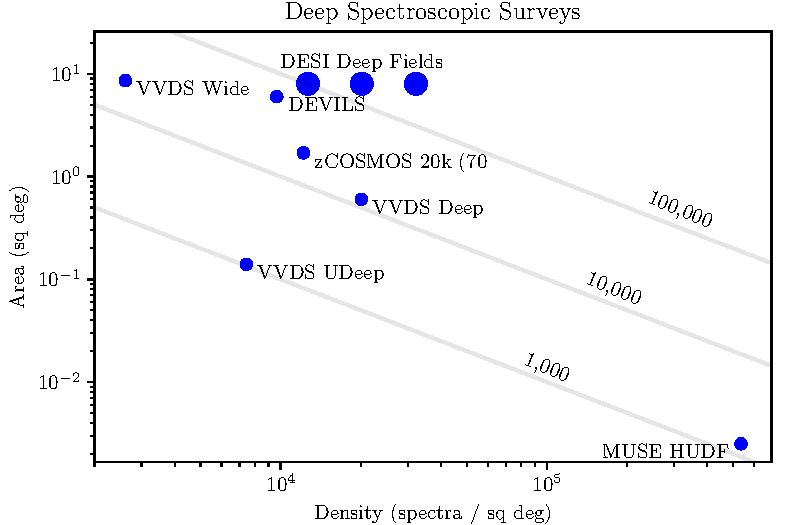
\includegraphics[width=0.5\textwidth]{deep-spec}
  \end{center}
  \caption{Deep spectroscopic surveys, by area and density.  The
    diagonal lines show constant total number of spectra.  The DESI
    Deep Fields proposed here (the three markers indicate $r$-band
    limits of $23.0$, $23.5$ and $24.0$) surpass existing surveys,
    opening up a new region of wide area and target density.
    \label{fig:surveys}}
\end{figure}

% As shown in Figure \ref{fig:surveys}, the proposed DESI Deep Fields
% would surpass available deep spectroscopic surveys in area, depth,
% and target density.


% DES SN fields
% CDFS (Dec -28)
% ELAIS-S1 (Dec -43)
% XMM-LS (36.45, -4.6)
% STRIPE2 (42.75, 0.0)

\section{Detailed request}

During DESI survey validation, we propose observing the \textbf{COSMOS} field,
centered near RA,Dec = $(150.0, 2.2)$.
This field has many positive features:
\begin{itemize}[noitemsep]
\item one of two LSST Deep-Drilling Fields reachable by DESI (the other is XMM-LSS) 
\item \emph{Euclid} calibration field
\item observable during likely SV timeline
%\item equatorial
\item very rich multi-wavelength imaging observations, yet
  surprisingly sparse public spectroscopic observations
\item deeper-than-average coverage in Legacy Surveys DR8/DR9, with
  \emph{considerably deeper} imaging available
\end{itemize}

In addition, we expect that several other DESI secondary programs will
wish to target COSMOS, and this program can very naturally interleave
with other programs.

\paragraph{Target selection}
During SV, we propose the simplest possible target selection
criterion: a simple $r$-band total magnitude cut on the Legacy Surveys
standard catalogs.  We will include point-like sources in order to
observe all AGN.

We expect that a fibermag cut may be required to eliminate
low-surface-brightness galaxies, and we expect to tune some additional
cuts, based on what we learn during SV based on the simplest magnitude
cut.

The density of targets (that we might observe over the course of
several years) is very large, depending on the magnitude limit as
detailed in Table \ref{tab:targets}.  This is based on extrapolating
the Legacy Surveys DR8 catalogs covering the one square degree in the
core of COSMOS.  This catalog is complete to \emph{about} $r=23.9$, so
the $r=24$ is a slight underestimate.  We list the target density, the
density of targets that are classified as ``PSF'' in the DR8 catalogs,
the percentage of poinit sources, and finally, the approximate number
of DESI tilings this density would require, assuming 10\% overhead.
We also include $r<20$ targets, which we would request to do during
bright time.

\begin{table}
\begin{tabular}{|c|r|r|r|r|}
  \hline
  \textbf{r-band limit} & \textbf{targets/sq.deg} & \textbf{point sources/sq.deg} & \textbf{\% point sources} & \textbf{DESI tilings} \\
  \hline
  20.0 & 4,000  & 2,500 & 63\% & 7 \\
  22.0 & 14,500 & 5,300 & 36\% & 26 \\
  22.5 & 20,200 & 6,300 & 31\% & 36 \\
  23.0 & 28,500 & 7,800 & 27\% & 50 \\
  23.5 & 40,800 & 10,400 & 26\% & 72 \\
  24.0 & 57,600$^\ast$ & 16,000$^\ast$ & 28\% & 101 \\
  \hline
\end{tabular}
\caption{Target densities for magnitude-limited samples of increasing depth.
  We include the number and fraction of these targets that are point sources,
  and the appoximate number of DESI tilings required. \label{tab:targets}}
\end{table}
% At r < 20.0, 3956 total, 2480 PSF, 62.7 % PSF; 7.0 DESI tilings
% At r < 22.0, 14462 total, 5265 PSF, 36.4 % PSF; 25.5 DESI tilings
% At r < 22.5, 20205 total, 6324 PSF, 31.3 % PSF; 35.6 DESI tilings
% At r < 23.0, 28467 total, 7797 PSF, 27.4 % PSF; 50.1 DESI tilings
% At r < 23.5, 40761 total, 10400 PSF, 25.5 % PSF; 71.7 DESI tilings
% At r < 24.0, 57622 total, 16018 PSF, 27.8 % PSF; 101.4 DESI tilings

\paragraph{SV target selection}
During SV, we aim to characterize the redshift success rate
distribution (including sources for which the current spectroscopic
template set is insufficient; see below) as a function of depth and
exposure time.  Targets from other deep secondary programs can be used
for this purpose as well.  The results from SV will guide the
development of the final observing strategy.  In addition to exploring
additional cuts, a key quantity is our target redshift completeness
rate.  We do not want to continue spending exposure time on the tail
of sources that will never yield a redshift (some of which may be due
to imaging pipeline artifacts), but we do want to keep the
completeness as high as is practical.


\paragraph{Tiling} We will use David Schlegel's ``rosette'' strategy,
in which DESI tile centers are placed at points on a circle around the
field center with a radius $0.28$ deg, to spread out the DESI central
dead zone.  The number of tilings should not be a factor of 2 or 5 to
avoid DESI instrument symmetries.  For example, we could do 7-, 9-,
and 11-point dithers with different starting angles.  This yields a
flat-topped completeness function (each target can be reached by a
fiber in $> 80\%$ of tilings) out to diameter of $\sim 2.7$ degrees,
with the completeness ramping down smoothly.  We propose observing
dozens of tilings ultimately.

\paragraph{Observing strategy}  We propose a simple iterative observing
strategy.  We will update the target list periodically (not in real
time) as tiles are observed, retiring all targets that get a redshift.
Then, the observing strategy is simply: for each fiber, \emph{observe
  the brightest target reachable that does not already have a
  redshift, and that we have not already observed this round.}  We
will choose a ``unit'' exposure time (for example, 30 or 60 minutes)
for the individual tilings.

\paragraph{Redshift fitting}
Since our sample will be much broader than the core DESI cosmology
sample, we will need to expand the galaxy template set used by the
spectroscopic pipeline.  John Moustakas has committed to performing
this task, which will then benefit the main survey as well as other
secondary programs.



\bibliography{desi-deep}{}
\bibliographystyle{aasjournal}

\end{document}


